\yesmargins
\chapter{Project Management \& Teamwork}

\begin{tikzpicture}[overlay,remember picture] 
\node[anchor=south] at ([yshift=5in,xshift=0.85in]current page text area.south){\includegraphics[width=9in]{pjm03}}; 
\end{tikzpicture} 

\marginpar{\projectManagementDef\margindivider}\marginpar{\tripleConstraintDef}\textbf{Project management}\index{project management} is the process of planning and executing a project while balancing the time, cost, and scope constraints. Time, cost, and scope are known as the \textbf{triple constraint}\index{triple constraint}\index{constraints}\index{project constraints}.

How does one minimize time and money spent on a project while delivering an adequate feature set? Risk management\index{risk management}\index{risk mitigation} is key. \textbf{Risk}\index{risk} is the estimated probability of a loss given a set of known and unknown factors. Risk can be stated as high, medium, or low, or numerically. Ways to mitigate risk include \textbf{defining and keeping track of your project}, \textbf{communicating} with your project team, researching the \textbf{implications} of decisions, developing \textbf{backup plans}, and selecting suitable \textbf{tools}. 

This chapter covers a variety of project management\index{project management} methods, including those related to \textbf{teamwork}\index{teamwork}. None of them are limited to just one type of software development environment but this chapter, like all of this book, is slanted toward \marginpar{\riskDef\margindivider}\marginpar{\contingencyDef\margindivider}Agile\marginpar{\agileDef}. There are many more methods that aren't discussed here; instead of hoping to be comprehensive, this chapter gives you a starter set of methods that are well known and highlight different areas of project management.

\section{Why learn about project management?}

Since this book is aimed at people who want to become or are software engineers, why is there a chapter about project management? Reasons to learn project management:\\
\begin{itemize}
    \item You might \textbf{become} a project manager (e.g., because your employer asks you to fill the role or you're interested).\\
    \item You might \textbf{have} a project manager. Understanding some basics of project management can help you understand what they're doing (e.g., using a RACI matrix\index{RACI matrix} to define who on the team does what) and what they're trying to tell you about the project (e.g., implications of the burn down chart analysis).\\
    \item You might need to \textbf{self-manage} (e.g., within an organization that has a flattened hierarchy or within an Agile\index{agile} team).
\end{itemize}

\section{Triple Constraint}\index{triple constraint}\index{project constraints}\index{constraints}

Project management\index{project management} is partially about \textbf{optimization}\index{optimization}: How can we use our limited financial and personnel resources to complete our project by the deadline, without going over-budget? These concerns are often summarized as needing to balance three constraints:

\begin{itemize}
    \item \textbf{Time}\index{project duration}: Duration of the project, intermediate deadlines
    \item \textbf{Cost}\index{project cost}: Monetary, personnel, and other project resources
    \item \textbf{Scope}\index{scope}\index{project scope}: What the project is meant to accomplish and the requirements of the project, including quality.\marginpar{Other authors in other fields sometimes consider quality separate from constraint. In software engineering, requirements\index{requirements} include quality.}
\end{itemize}

This set of three is called the \textbf{triple constraint}\index{triple constraint}\index{constraints}\index{project constraints}.

It can be difficult to balance these three constraints. Common challenges:

\begin{itemize}
    \item You're meeting with a client and they say, ``Oh I forgot to mention we want this feature, that won't be a big deal, right?'' (affects \textbf{scope})
    \item You realize late in the project that, to implement feature A, you'll need to implement B, C, and D as well. (affects \textbf{cost})
    \item Your team's estimates were overly optimistic. (affects the \textbf{time} constraint\index{project duration})
\end{itemize}

These situations are so common that you can \textbf{assume they're going to happen} and come up with a \textbf{mitigation plan}\marginpar{\mitigationPlanDef}\index{mitigation plan} even before the project starts. But many situations are more complicated (more factors with more interrelationships), more unique to your context, and have factors that leak from your professional life to your personal life. Examples: \\

\begin{itemize}
    \item You're working on a project with a friend, who is an excellent coder but only available for the next three months (\textbf{time}). They also have their own ideas about where they want the project to go (\textbf{scope})\index{scope}\index{project scope}. You know your friend will be more enthusiastic about the project if they have more control, and that means quicker implementation and less work for you (\textbf{cost})\index{project cost}. But that'd mean sacrificing some of your own feature priorities (\textbf{scope}). \\
    \item You're working with a five-person team. Your colleague needs help but all hours must be billed to a project, you're getting pressured to stay close to the budget, and you bill at a higher rate than your colleague (\textbf{cost}). If your colleague doesn't get help, they might spend extra hours self-training (\textbf{cost}), might switch to a different project, and there's a small chance they'll make the project take longer (\textbf{time}). \textbf{Scope} is fixed: The product must satisfy all its requirements. \\
\end{itemize}

Making strategic project decisions involves adjusting project constraints\index{constraints}\index{project constraints}. If you want to reduce time and cost spent on a project or increase project scope, you'll need a corresponding change in one or more other constraints. One way to visualize this:
\begin{itemize}
    \item Begin with an \textbf{equilateral triangle}. The three edges represent time, cost, and scope. Time and cost are already as small as possible. Scope is as large as possible, given the time and cost constraints.
    \item If you want the project to take less time (shorter time edge), you'll have to either increase the length of the cost edge, make the scope edge shorter, or do both. Likewise with adjusting the other constraints.
    \item This model only goes so far. Don't, for example, get caught up with trying to keep the area or perimeter of the triangle constant.
\end{itemize}
\marginpar{The triple constraint triangle (a.k.a. project management triangle) is sometimes shown with each vertex labelled instead of each edge. However, that triangle isn't as useful for imagining the impact of your project decisions.}

\begin{center}
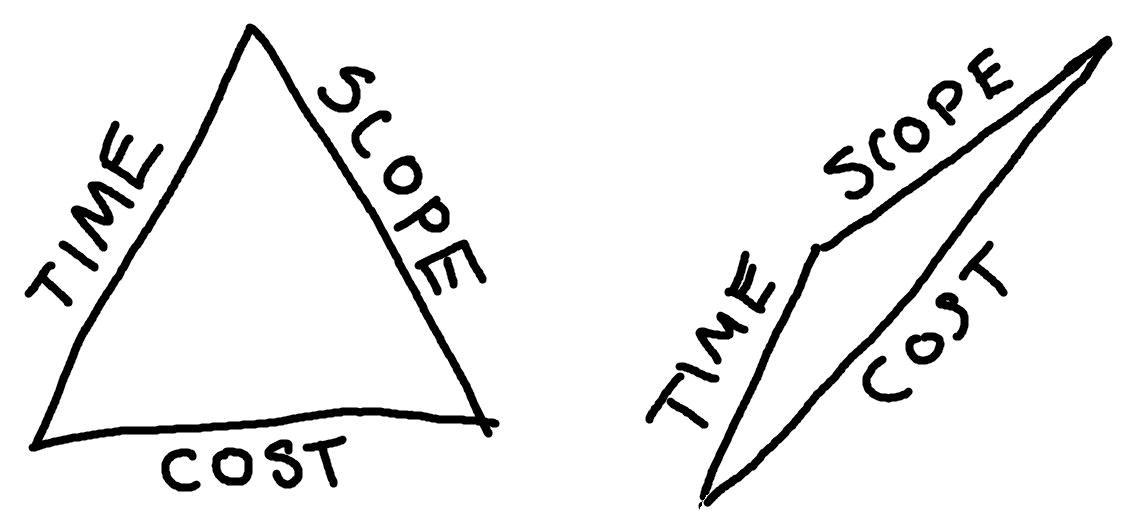
\includegraphics[width=\textwidth]{triangle}
\end{center}

\textit{If you want your project to take less time, you might have to tolerate it costing more or having a reduced scope.}

\section{Managerial Skill Mix}
\marginpar{\msmDef\margindivider} What skills are required for managing a project? There are three broad categories comprising the \textbf{managerial skill mix (MSM)}\index{managerial skill mix}\index{MSM (managerial skill mix)}:
\begin{itemize}
    \item \textbf{Interpersonal}\index{interpersonal skills}: Communicating effectively with anyone likely to affect the project (e.g., engineers on your team, managers, clients, contractors, IT support, etc.)
    \item \textbf{Technical}\index{technical skills}: Using \textbf{methods}\marginpar{\methodDef} and equipment effectively (e.g., knowledge of appropriate processes, understanding and writing code, etc.)
    \item \textbf{Administrative and conceptual}\index{administrative skills}\index{conceptual skills}: Understanding the ``big picture'' vision (conceptual) and being able to move macro-level pieces (e.g., teams, departments, divisions, etc.) toward that vision (administrative).
\end{itemize}
High-level managers (e.g., CEOs) tend to need a different mix of skills than lower-level managers (e.g., project managers). For example, a project manager might need strong interpersonal and technical skills while only occasionally considering the big picture of how a project fits into organization's overall vision. Since this chapter is about project management, we will focus more on interpersonal and technical skills.

\section{Interpersonal Skills: Team Communication}

One way to reduce risk is to \textbf{improve team communication}\index{teamwork}\index{team communication}, which can increase the likelihood of project success.

As background for while you read this section, consider \textbf{Tuckman's\marginpar{\tuckmanDef}\index{Tuckman's five stages of team development} five stages of team development}:

\begin{enumerate}
    \item \textbf{Forming}\index{team formation}\index{forming (Tuckman's model)}: Team members become oriented through testing each other's boundaries and establishing dependency relationships with peers, leaders, and existing team standards.
    \item \textbf{Storming}\index{storming (Tuckman's model)}: Team members resist group influence, their peers, their peers' ideas, and tasks.
    \item \textbf{Norming}\index{norming (Tuckman's model)}: Team develops cohesiveness, new team standards and roles, and team members express personal opinions related to tasks.
    \item \textbf{Performing}\index{performing (Tuckman's model)}: Team roles\index{team roles} become flexible, team dynamics\index{team dynamics} and structure serve the function of the team and task performance\index{task performance}.
    \item \textbf{Adjourning}\index{adjourning (Tuckman's model)}: Team disbands.
\end{enumerate}

The rest of this section will discuss specific methods a team can use to improve communication\index{team communication}. Consider where each might fit in to these stages (there's not just one answer).

\subsection{Establishing Ground Rules}

Team \textbf{ground rules}\index{ground rules}\index{communication ground rules}\index{team ground rules} are a preemptive or reactive method for reducing team conflict\index{team conflict} and dysfunction. Ground rules might already exist when a team forms, others might develop as the team becomes normalized, and revisions might happen as the team proceeds with their work and identifies new team concerns or opportunities. To be effective, the ground rules need buy-in from the whole team. What the ground rules should cover or should be varies by team, but here are questions teams can discuss to help:
\begin{itemize}
    \item \marginpar{\groundRulesDef\margindivider}\marginpar{When deciding on ground rules\index{ground rules}\index{team ground rules}, your team might choose to incorporate ground rules or standards already established by others, such as the IEEE Code of Ethics\index{IEEE code of ethics} or the Agile Manifesto\index{agile manifesto}.\margindivider}\marginpar{If your team was to start with a single ground rule, what would be a good one? Maybe, ``We agree to discuss adding more ground rules as needed.''}What is our \textbf{vision} for what this team is or what we're trying to accomplish together? (e.g., clients choose us because we're honest and transparent)
    \item What do we \textbf{prioritize} most?\index{team priorities} (e.g., delivering a high-quality product ahead of the deadline, input from all team members, honoring diverse end-users, making the big bucks, etc.)
    \item What methods will we use for \textbf{day-to-day communication}\index{team communication}? (e.g., no interrupting, no 'splaining, listen to and acknowledge what other people are saying, ask people if they're busy before starting a long conversation, etc.)
    \item What methods will we use \textbf{communicate} with each other \textbf{during} \textbf{conflict}? (e.g., we'll get trained on and use non-violent communication)
    \item What expectations do we have for \textbf{work habits}\index{team work habits}? (e.g., 1 to 3pm on Tuesday is silent time, be 5 minutes early to meetings, etc.)
    \item What expectations do we have for \textbf{responsiveness}\index{team responsiveness}? (e.g., respond within 2 hours during regular work hours and within 24 hours over the weekend, have the team Discord open during regular work hours, etc.)
    \item What will we do when team members \textbf{fail expectations}\index{team expectations}? (e.g., we'll discuss any team problems Friday at 3pm, etc.)
    \item How will we \textbf{get to know each other}? (e.g., we'll discuss each other's cognitive styles, we will not flirt with each other, we will have bring-your-pet-or-child to work days, etc.)
\end{itemize}

The end product of answering questions like these could be a list of short statements that's posted somewhere people will see it regularly. 

The questions your team asks, and the answers, will vary depending on the individuals on the team and on context (e.g., culture). Whatever those questions and answers are, ideally they will feel meaningful and authentic. If your team gets the feeling the ground rules\index{ground rules} are silly, phony, too aspirational, too inflexible, too authoritative, etc., that could invalidate your team's efforts toward creating the ground rules.

\subsection{Defining Roles and Responsibilities: RACI Matrix}\index{RACI matrix}\index{team roles}\index{team responsibilities}
\marginpar{\raciMatrixDef\margindivider}\marginpar{\mvpDef\margindivider}\marginpar{\focusGroupDef}A RACI matrix is a chart for defining who is responsible (R) and accountable (A) for a task or deliverable and who should be consulted (C) or informed (I). \\

\noindent\textbf{Basic example} defining who should do what during the minimum viable product (MVP) development phase:
\begin{center}
\rowcolors{0}{white}{white}
\begin{tabular}{c|c|c|c|c|c|c|c|}
    & \rotatebox[origin=l]{90}{Frontend Developers} & \rotatebox[origin=l]{90}{Frontend Designers} & \rotatebox[origin=l]{90}{Frontend Lead} & \rotatebox[origin=l]{90}{Backend Developers} & \rotatebox[origin=l]{90}{Backend Lead} & \rotatebox[origin=l]{90}{Team Lead} \\
    \hline
    \rowcolor{light-gray}
    \textbf{Phase 1: MVP} &  & & & & & \\
    \hline
    Focus groups & C & R & R / A & C & C & R / A \\
    \hline
    Requirements spec. & R & R & A / I & R & A / I & C \\
    \hline
    Throwaway code design & & & I & R & A & I \\
    \hline
    Implementation & R & C & A & R & A & C \\
    \hline
    User acceptance testing & R & R & R / A & R & C & C
\end{tabular}
\end{center}
\textbf{Interpreting a RACI matrix}:\index{RACI matrix}
\begin{itemize}
    \item Top row: Roles. One person might have multiple rows.
    \item First column: Tasks or deliverables, organized into phases (if needed). 
    \item Letters define what role is responsible for which task or deliverable.
    \item \textbf{Responsible (R)}: Who will do the work
    \item \textbf{Accountable (A)}: Who will approve the work and make sure it gets done
    \item \textbf{Consulted (C)}: Who can discuss and offer advice about the work
    \item \textbf{Informed (I)}: Who to keep up-to-date about the status of the work
\end{itemize}

A RACI matrix\index{RACI matrix} is a method for reducing risk\index{risk mitigation}: If your team doesn't know who needs to do what (or forgets, or can plausibly deny knowing), that can increase the probability of a negative events and outcomes (e.g., shipping a broken product to customers because nobody was assigned to quality assurance).

\subsection{Measuring and Building Consensus: Fist of Five Method}
\textbf{Fist of five}\index{fist of five}\index{consensus building}\index{teamwork} is a method for checking and building consensus within a group of people. One person (e.g., team leader) makes a statement or proposes an idea to a group and each person communicates their level or agreement or support by holding up a first or up to five fingers. It has become associated with Agile\index{agile} \parencite{belling2020agile}, but I've also seen examples of it being used with students of different ages (e.g., \parencite{fletcher2002firestarter}, \parencite{hulshult2019using}). \textbf{What each number of fingers means}:\marginpar{\fistOfFiveDef\margindivider}\marginpar{Meanings of single-finger hand gestures vary around the world. For example, in the US putting your thumb up means ``good job'', in Australia, Greece, and the Middle East it means ``up yours'', in Germany and Hungary it means ``one'', and in Japan it means ``five''! \parencite{cotton2013gestures}}

\begin{itemize}
    \item \textbf{None}: Strong reject. Blocks consensus.
    \item \textbf{One}: Reject. Major issues need resolving now.
    \item \textbf{Two}: Weak reject. Minor issues need resolving now.
    \item \textbf{Three}: Weak accept. Minor issues, can resolve later.
    \item \textbf{Four}: Accept. No issues.
    \item \textbf{Five}: Strong accept. Willing to lead or champion.
\end{itemize}

If anyone suggests rejecting the statement or idea by holding up two or fewer fingers, the team can stop, discuss, make changes, and re-vote until there's sufficient consensus. It's up to the team or its leader to decide how much consensus is needed.

The fist of five\index{fist of five} method can reduce risk\index{risk mitigation} by (1) bringing problems to light and (2) increasing team motivation\index{team motivation}, ownership\index{team ownership}, and investment\index{team investment}.

\section{Technical Skills: Project Definition}

This section contains methods for helping with the \textbf{technical side} of defining a project, including \textbf{prioritization}\index{prioritization}, \textbf{estimation}\index{estimation}, \textbf{scheduling}, and \textbf{task management}\index{task management}.

\subsection{Project Scope}\index{project scope}
In an \textbf{Agile software development environment}\index{agile}, a project's scope is implied through sets of tasks (e.g, release plan\marginpar{\releasePlanDef\margindivider}\index{release plan}, Product Backlog\marginpar{\productBacklogDef\margindivider}\index{product backlog}, iteration plan\marginpar{\iterationPlanDef\margindivider}\index{iteration plan}, Sprint Backlog\marginpar{\sprintBacklogDef\margindivider})\index{sprint backlog}. Each iteration might have a goal (e.g., a Sprint Goal)\index{sprint goal} that summarizes what the set of tasks is meant to accomplish, which is also part of defining scope for Agile\index{agile} projects. The scope is purposely flexible and emerges as the project proceeds.

In \textbf{other environments}, the project scope (a.k.a. statement of work)\index{statement of work} is a specific document stating the project's objective, deliverables (outputs), milestones, technical requirements, and limitations/exclusions. 

\subsection{Balancing Constraints: Project Priority Matrix}\index{constraints}\index{project priority matrix}\index{priority matrix}
Earlier, we talked about the three major constraints of project management\index{project management}\index{project duration}\index{triple constraint}\index{project cost}\index{project scope}---time, cost, and scope---and that balancing them isn't always straightforward. What should the balance be? How do I know whether I'm achieving balance? How does this fit into how the project is run? One method for more concretely stating the desired balance is the \textbf{project priority matrix}\marginpar{\projectPriorityMatrixDef}\index{priority matrix}\index{project priority matrix}:
\rowcolors{0}{white}{white}
\begin{center}
\begin{tabular}{r|c|c|c}
    \rowcolor{light-gray}
    & Time & Cost & Scope \\
    \hline
    Constrain & & & \\
    \hline
    Enhance & & & \\
    \hline
    Accept & & &
\end{tabular}
\end{center}
\begin{itemize}
    \item \textbf{Constrain}: The constraint is fixed (can get better but must not get worse)
    \item \textbf{Enhance}: Try to improve (e.g., take less time, spend less, have more features)
    \item \textbf{Accept}: Can worsen (e.g., more time, more personnel, fewer features) if necessary
\end{itemize}
For \textbf{example}, if you have a grant from the National Institutes of Health (NIH) to write and test software for a medical device that automatically regulates a person's pain level, your project priority matrix might look like this:
\begin{center}
\begin{tabular}{r|c|c|c}
    \rowcolor{light-gray}
    & Time & Cost & Scope \\
    \hline
    Constrain & & & \checkmark \\
    \hline
    Enhance & & \checkmark & \\
    \hline
    Accept & \checkmark & &
\end{tabular}
\end{center}
\textbf{Scope}\index{project scope}\index{scope}: Fixed. Your team must do what they said they'd do, and cannot scrimp on quality. If the device only partially works, that would be a disaster---you'll be testing it on human subjects! \textbf{Cost}\index{project cost}: Needs to be tightly controlled because the grant is for a fixed amount and funded by taxpayers. \textbf{Time}: While hopefully the project stays on track and delivers as promised, if needed your team can submit intermediate results to the NIH and (hopefully) use those results to get another grant.

Ideally, the project priority matrix\index{project priority matrix}\index{priority matrix} would be defined before the project starts (with the client) and referenced throughout the project as needed. Developing and adhering to the matrix can reduce risk\index{risk mitigation} by helping the team or project manager balance constraints in ways that are acceptable to the client.

\marginpar{\eisenhowerMatrixDef\margindivider}\marginpar{\blockquote{I have two kinds of problems, the urgent and the important. The urgent are not important, and the important are never urgent.} --Dwight D. Eisenhower \margindivider}\marginpar{\extremeProgrammingDef\margindivider}\marginpar{\scrumDef}\subsection{Task Prioritization: Eisenhower Matrix}\index{Eisenhower matrix}\index{task prioritization}\index{prioritization}

Individual tasks, too, need relative prioritization. In an Agile\index{agile} \textbf{Scrum}\index{scrum} environment, this would be the responsibility of the \textbf{Product Owner}\index{product owner} and in Agile\index{agile} \textbf{Extreme Programming (XP)}\index{extreme programming (XP)} it's the customer (i.e., someone representing the customer, like the \textbf{client})\index{client}. 

But how are task priorities\index{task prioritization} decided? One high-level method is called the \textbf{Eisenhower matrix}\index{Eisenhower matrix}:

\begin{center}
\begin{tabular}{c|c|c}
    & Urgent & Not Urgent \\
    \hline
    Important & \textbf{Do} & \textbf{Decide} \\
    \hline
    Not Important & \textbf{Delegate} & \textbf{Delete}
\end{tabular}
\end{center}

\begin{itemize}
    \item \textbf{Do} (urgent, important): Needs to be done correctly and now. \textbf{Example}: Documenting your undocumented code so that a new hire can start contributing.
    \item \textbf{Decide} (not urgent, important): Needs to be done correctly but not immediately. \textbf{Example}: Refactoring your currently-working code. Needs to be done eventually, and done right---maybe the new hire can handle it in a couple months.
    \item \textbf{Delegate} (urgent, not important): Needs to be done now but mistakes can be absorbed (e.g., tolerated, corrected later, etc.). \textbf{Example}: Someone needs to initialize the task management system so the team can begin defining tasks. If it's not done right, that's fine---the developers and managers will adjust the setup as needed. Good learning task for the new hire, who doesn't have much to do right now.
    \item \textbf{Delete} (not urgent, not important): Doesn't need to be done correctly or any time soon. Can be eliminated. \textbf{Example}: Implementing a loading screen that looks like a game of pong, but you're the only one on the team who thinks that's a cool idea. 
\end{itemize}
Doing a first-pass task prioritization\index{task prioritization} using an Eisenhower matrix\index{Eisenhower matrix} can reduce risk\index{risk mitigation} by both \textbf{conserving resources} and using them \textbf{thoughtfully} (including yourself). It can also help with getting out of the mode of ``putting out fires'' (concentrating on the urgent tasks), which can result in important but non-urgent tasks getting eternally left at the end of the to-do list (perhaps resulting in project failure).

\subsection{Finer-Grained Prioritization}\index{task prioritization}

What happens when there are \textbf{multiple important tasks} to complete that have the \textbf{same level of urgency}? How does one decide which is more important? \textbf{Some methods} for deciding which task has higher priority when they seem roughly equivalent:\\

\begin{itemize}
    \item For implementation tasks (e.g., coding, architecture, other implementation choices, etc.), \textbf{ask an expert}. They might know from past experience which tasks have more unknowns, more risk, dependencies, etc.\\
    \item If it's an implementation task and you're meant to be an expert, you can do a \textbf{focused research effort called a spike}\marginpar{\spikeDef}\index{spike} to gather more information about the task, which in turn can help you prioritize it. To do a spike: (1) Come up with a question, (2) Focus on answering the question, discovering additional questions and sub-questions in the process, (3) Repeat until you have enough information. A good way to do a spike\index{spike} is to start doing the task and see what obstacles you run into. \textbf{Example}: You need to set up a local server for testing and write a test suite. You have experience writing a test suite but have never set up a server. After doing a spike, you realize that some of the tests you're going to write rely on the local server have a static IP address, which you learned is not the default. Based on your findings, you decide to prioritize the server setup because (1) the test suite strongly depends on it and (2) the server setup task still has many unknowns and you're not sure how long it'll take to eliminate those. \\
    \item Think about \textbf{dependencies}: Who is waiting on you? How many other tasks depend on this task? Compare that to the important of the dependent tasks (or the importance of keeping the waiting person happy / productive) and how long it'll take to complete the task. \textbf{Example}: You estimate it'll take 15 minutes to complete a task that two other people are waiting on. You decide to do that before your 4-hour task. Seems like the obvious choice---but if you're not aware of which tasks depend on yours or are deep into solo work mode, you might make a sub-optimal choice.\\
    \item If you're deciding which feature to implement, you can \textbf{ask the customer or users} directly (e.g., through a phone call, focus groups\marginpar{\focusGroupDef\margindivider}\index{focus group}, usability testing\index{usability testing}\marginpar{\usabilityTestingDef\margindivider}\marginpar{\estimationDef\margindivider}\marginpar{\storyPointsDef}, etc.) or indirectly (e.g., by looking at support tickets, asking the marketing team, detecting an unmet need based on how people use other software, etc.).\\
    \item Other ways to select features: \textbf{Voting} (e.g., within your team) or \textbf{pairwise comparison} (e.g., Is Feature A more valuable than Feature B? If so, is Feature C more valuable than Feature A?).\\
\end{itemize}
A natural side effect of prioritization\index{task prioritization} is finding how long it'll take to complete a task, what dependencies exist, who the players are, and what the end user wants: All this knowledge contributes to risk mitigation\index{risk mitigation}.

\subsection{Estimation: Story Points, Ideal Days, and Planning Poker}
Intertwined with prioritization is \textbf{estimation}\index{estimation}: Figuring out ahead of time how long a task is likely to take. But what does ``how long'' mean and how do we figure out ``how long''?

\textbf{Two methods}, from the Agile community, of \textbf{stating the size of a task}:

\begin{enumerate}
\item \textbf{Story points}\index{story points}: Assign a number to a task representing its size relative to other tasks. For example, a software installation and a virus scan might both be a 1 if they take roughly the same amount of time and effort, have roughly the same amount of risk, etc. Implementing a major feature might, on the other hand, be an 8. Your team decides how far the scale goes.\marginpar{Common scales for story points: 1 to 10, Fibonacci, and powers of two. The latter two are meant to help make sizing a task easier by putting more distance between the numbers in the scale: Deciding between a 4 and an 8 can be easier than deciding between a 4 and a 5.\margindivider}\marginpar{\idealDaysDef}
\item \textbf{Ideal days}\index{ideal days}: Assign a number of days you think it'd take to complete the task if there were no other tasks, no distractions, etc. For example, if it takes me 5 minutes to remove one square foot of grass from my lawn, and I have 100 square feet to remove, that is 8 hours and 20 minutes total, so about one ideal day (if your work days are eight or nine hours).
\end{enumerate}

Once story points\index{story points} or ideal days\index{ideal days} are assigned, a team can make statements like, ``This month, we will complete 50 story points'', ``10 ideal days'', etc. Work completed (in story points or ideal days) is, in Agile teams, called the \textbf{velocity}\marginpar{\velocityDef\margindivider}\index{velocity}\index{project velocity}. Teams can make initial estimates about velocity then adjust depending on how accurate those estimates end up being.

But \textbf{how are estimates assigned} to a task? Another Agile idea is \textbf{planning poker}\index{planning poker}\marginpar{\planningPokerDef\margindivider}\marginpar{\schedulingDef\margindivider}\marginpar{\projectNetworkDef}\index{project network}. With this method, the team gets together to discuss a set of tasks and each person gets a set of cards with the different possible story points / ideal days / etc. a task can be assigned. One person describes the task, the team asks questions as needed, and then each person privately decides on an estimate by selecting a card (keeping it face-down or hidden). Once everyone is ready, the cards are revealed. Variations in estimates are expected, and part of the process: differences open a discussion. Someone making a high estimate might, for example, have thought of good reasons why a task is likely to take a long time. Someone making a low estimate may have identified an efficient idea nobody else thought of. The team discusses and, once ready, can repeat the process until estimates become sufficiently consistent.

\subsection{Scheduling: Project Network}

Once a set of tasks has been defined, prioritized, and estimated, those tasks can be scheduled. \textbf{Scheduling}\index{scheduling}\index{task scheduling} a task is placing it within the timeline and context of a project. The context of a project includes other tasks, personnel, and non-personnel resources (e.g., equipment), and milestones\index{project milestones}. One method for defining and visualizing a project's schedule\index{project schedule} is using a \textbf{project network}\index{project network}. A project network is a directed graph showing a project's tasks, the sequence in which they're to be completed, and the dependency relationships between the tasks. The nodes in the digraph represent tasks and the lines with arrows represent dependency or sequence relationships. A project network moves left to right, where left is earlier in time.

\marginpar{This textbook does not cover strategies or methods for optimally assigning personnel or other resources to tasks.\margindivider}\marginpar{While complex project networks may be less valued in a Agile\index{agile} development environment, they might also be just the method you need for understanding a complex project.}For a task to be represented as a node on a project network, it needs to (at a minimum) be distinct from other tasks and its dependent tasks (a.k.a., predecessors) must be known. However, a project network\index{project network} becomes more useful if estimates for the tasks are also known.

\subsubsection{Constructing a Project Network}

Project networks\index{project network} can be created manually or automatically generated by software. If you want to include estimates in the project network, generating the network will likely be less cumbersome, especially since you might want to modify your tasks or estimates once you see how the network looks. If you don't care about entering estimates and just want to visualize the sequencing and dependency relationships between tasks, drawing the network by hand might be sufficient for your needs.

For automatically generating a project network\index{project network} using software (e.g., MS Project, Lucidchart), you'd use the software's user interface to enter the task details. For example, in a table:

\begin{center}\marginpar{In Agile, predecessors are also called \textbf{blockers}\index{blockers} or \textbf{impediments}\index{impediments}, especially in cases when an activity could be started but is waiting on another activity (or external event) to occur.}
\begin{tabular}{c|c|c|c}
\rowcolor{light-gray}
Task ID & Task & Predecessors\index{predecessor}\index{task predecessor} & Duration \\
\hline
4 & Implement GUI & 1,3 & 50hrs \\
\hline
3 & Test GUI design with users & 2 & 5hrs \\
\hline
2 & Prototype GUI & & 8hrs \\
\hline
1 & Select GUI framework & & 2hrs \\
\end{tabular}
\end{center}

Note that, even though Task 2 must happen before Task 4, it's not listed as a predecessor because it's not an \textit{immediate} predecessor.

Depending on the software you choose for creating your project network\index{project network}, you might have access to more complex options like specific dates by which individual tasks must be completed.

\subsection{Task Management Systems}

A \textbf{task management system}\index{task management system}\marginpar{\taskManagementSystemDef} can be used to organize tasks, their details (e.g., description, acceptance criteria, assignee, status, etc.), and other relevant information (e.g., which iteration or phase the task belongs to). They're useful organizing and storing information about tasks, but also for the satisfaction of marking a task as done! Task management systems like Jira, Trello, and Asana are strongly oriented toward team collaboration. Some of these systems are also strongly Agile-oriented, in that they offer Agile-inspired features (e.g., templates). \textbf{Common features} of task management systems:

\begin{itemize}
    \item Create, remove, update, and delete tasks\marginpar{\projectManagementSystemDef\margindivider}\marginpar{\ganttChartDef}
    \item Enter task name, description, notes/comments, and add attachments
    \item View tasks as a list, as cards on a board, or within a timeline (e.g., Gantt chart)
    \item Organize tasks into projects
    \item Assign tasks to different team members, with due dates
    \item Enter task status (e.g., in progress, done)
    \item Get email notifications about tasks
    \item Add tags, keywords, and categories
\end{itemize}

Task management systems\index{task management system} don't universally have a way to generate project networks. For that, you might need a fully-featured \textbf{project management system}\index{project management system} (e.g, MS Project). However, you may find that a \textbf{Gantt chart}\index{Gantt chart} or roadmap feature meets your needs and is available within your task management system.

\section{Conclusion}
Project management and teamwork can reduce the risk of a project failing and make it possible to complete larger projects. Part of good project management is balancing time, scope, and cost.

\nomargins
\section{Additional Resources}

\begin{description}
    \item \fullcite{badawy1995developing}
    \item \fullcite{brennan2009guide}
    \item \fullcite{brown2013question}
    \item \fullcite{belling2020agile}
    \item \fullcite{cohn2005agile}
    \item \fullcite{cotton2013gestures}
    \item \fullcite{fletcher2002firestarter}
    \item \fullcite{hailes2014business}
    \item \fullcite{hambling2013user}
    \item \fullcite{hulshult2019using}
    \item \fullcite{jacka2009business}
    \item \fullcite{larson2013project}
    \item \fullcite{lucid2021fist}
    \item \fullcite{mahnivc2012using}
    \item \fullcite{mcalister2006project}
    \item \fullcite{microsoft2021triangle}
    \item \fullcite{overeem2016characteristics}
    \item \fullcite{stuart2014rules}
    \item \fullcite{tuckman1965developmental}
    \item \fullcite{tuckman1977stages}
    \item \fullcite{qubaisi2015leadership}
    \item \fullcite{usman2014effort}
    \item \fullcite{van2012theory}
    \item \fullcite{yang2011association}
\end{description}